\chapter{Localization techniques}\label{sec:LocalizationTechniques}
This chapter describes most common techniques and methods for localization. Most of these approaches have multiple implementations and can be also used in parallel. Fingerprinting for example can be used to increase accuracy of other methods.

\section{Triangulation}\label{sec:Triangulation}
Methods based on Triangulation use geometric properties of triangles to determine target position. This can further be divided into Lateration and Angulation \cite{RAinWILTaS}. There are multiple sources of data these methods can use like distance estimation between device and specific transmitters, measurements of the signal propagation-time (TOA: Time Of Arrival and TDOA: Time Difference of Arrival\cite{LTinWSN}) and the direction of received
signal (AOA: Angle of Arrival\cite{AoALforWSN}) \cite{IILUBLEB}.

\subsection{Lateration}\label{sec:Lateration}
Lateration refers to the technique of determining position based on distance measurements that are calculated using specific devices that know their own position.  Mainly used types of Lateration and are Trilateration and Multilateration. 

\begin{figure}[h!]
	\begin{centering}
		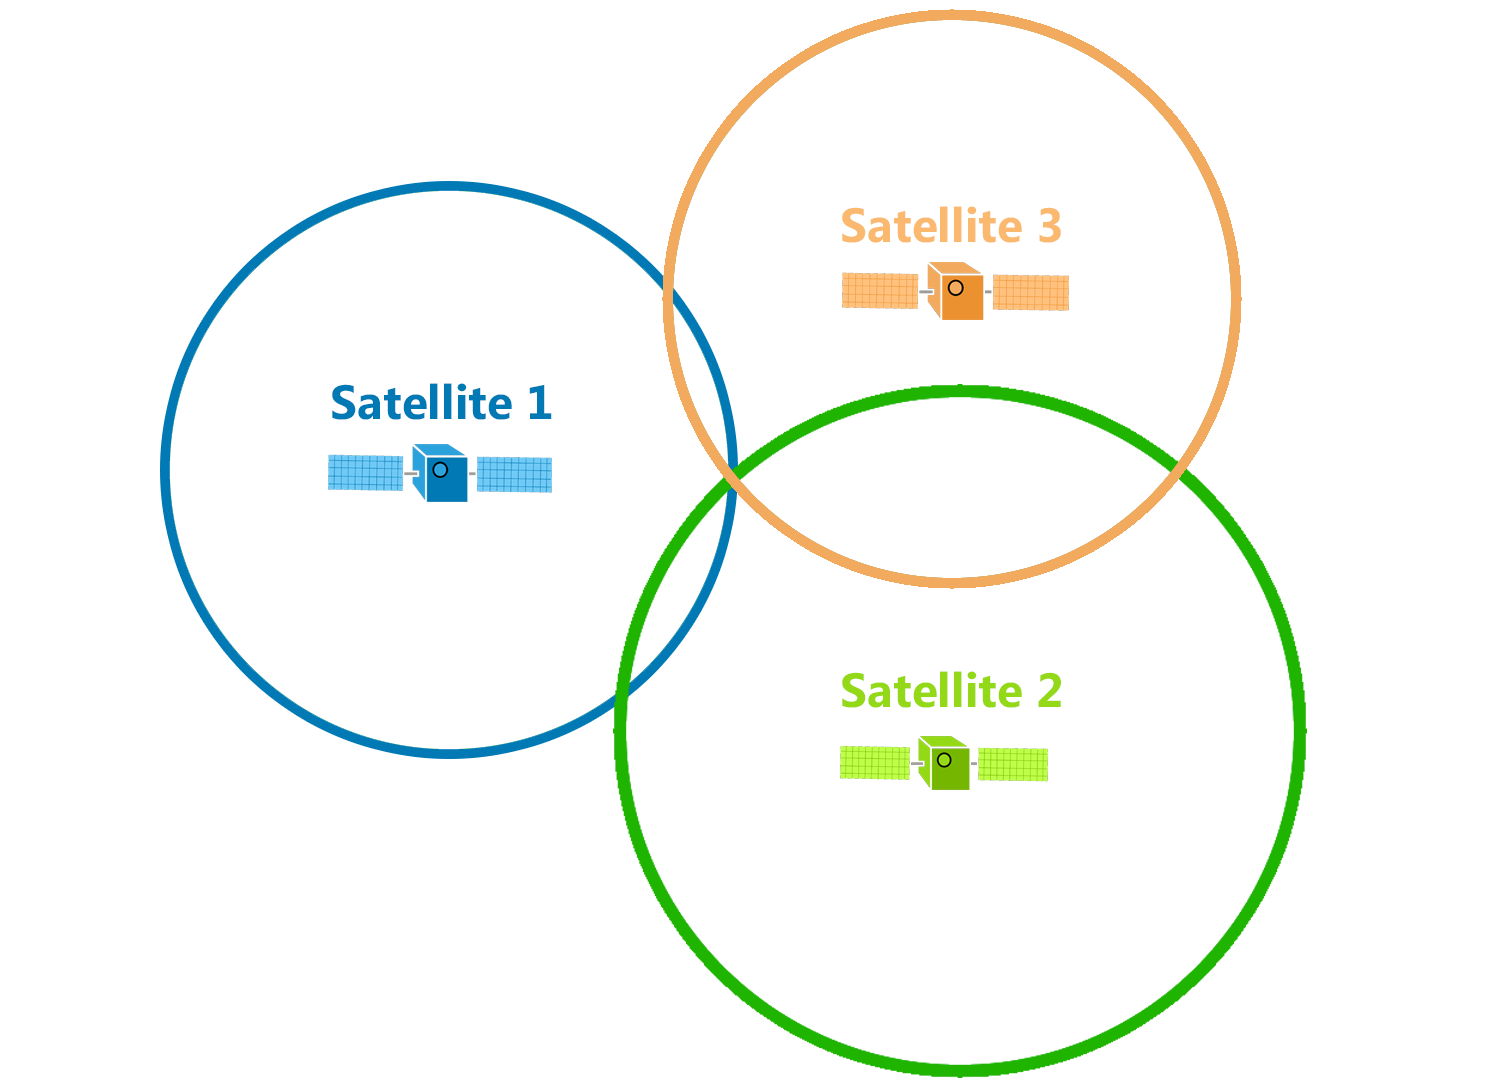
\includegraphics[width=0.48\textwidth]{img/trilateration_2d}
		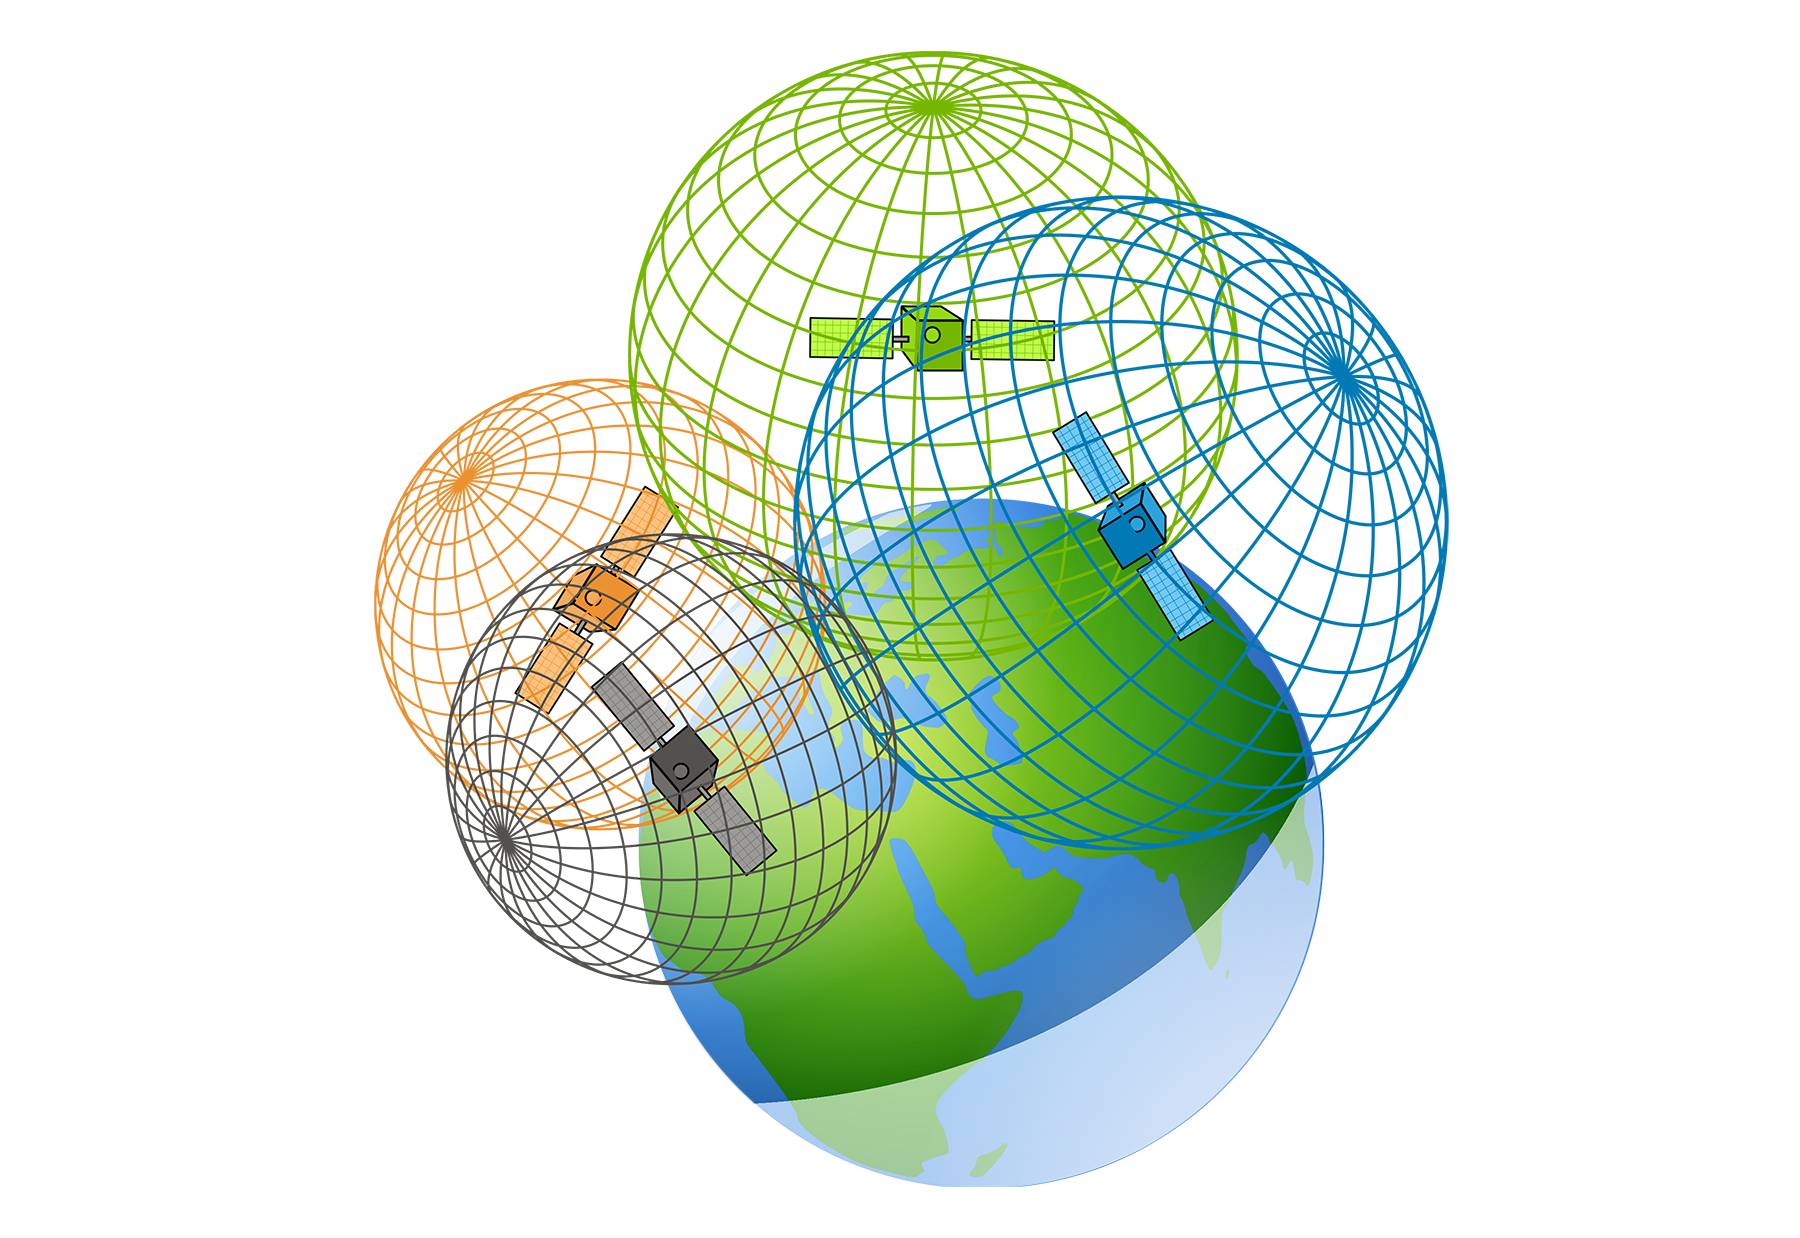
\includegraphics[width=0.48\textwidth]{img/trilateration_3d}
		\par\end{centering}
	\caption{2D and 3D Trilateration (source: \cite{TvTHGPSRW})\label{fig:2d_and_3d_trilateration}}
	\label{fig2}
\end{figure}

\textbf{Trilateration} uses distance measurements from at least three devices in particular as "tri" in the name suggests \cite{RAinWILTaS}. \fref{fig2} illustrates usage of Trilateration in 2D and 3D environment. While working in 2D plane will result with only one specific location point. Moving to the 3D plane can create a problem because signal is send in a sphere which could result in more than one position. That is the reason why some systems use at least four signal sources, example of such system is GPS \cite{GNSSGPS}. Advantage is easy implementation and simple calculations. One down side of this approach is that all devices must have synchronized clock \cite{RAinWILTaS}.

\medskip

\textbf{Multilateration} also known as hyperbolic positioning is using Time Difference of Arrival (TDoA) instead of Time Of Arrival (ToA) used in previous case. This approach involves the intersections of hyperbolas rather than circles as shown in \fref{fig3}. Main advantage of this method is that only receiving devices must have synchronized clock instead of all \cite{PLTaA}. Multilateration was developed for tracking aircraft position and it is widely used.

\begin{figure}[h!]
	\begin{centering}
		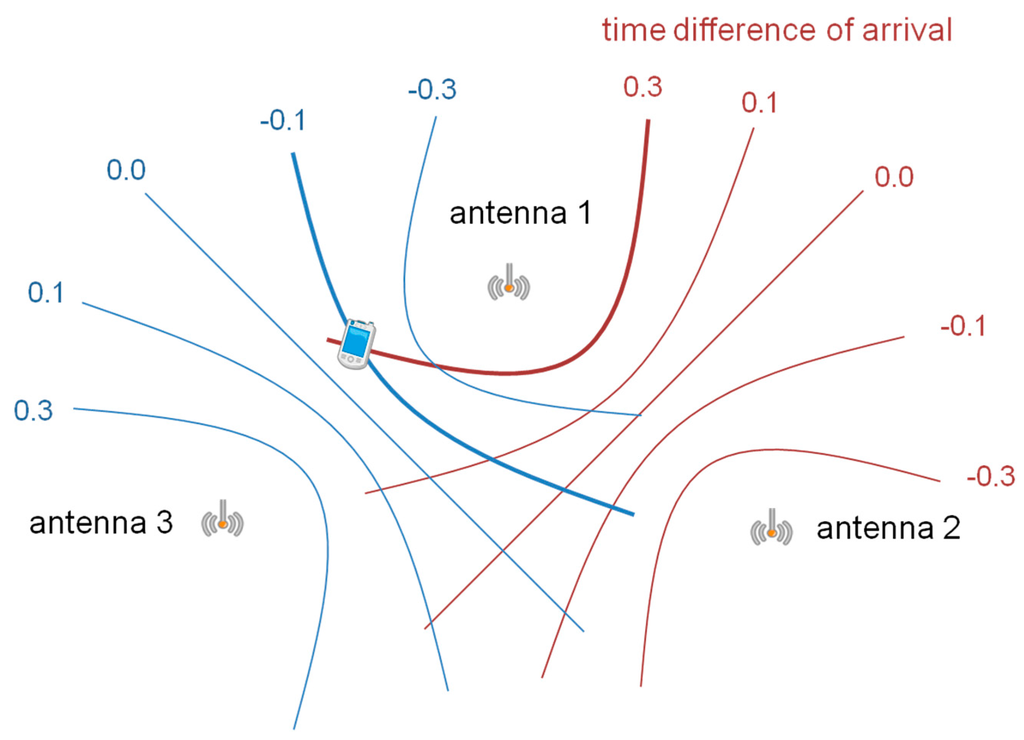
\includegraphics[width=0.6\textwidth]{img/multilateration}
		\par\end{centering}
	\caption{Multilateration (source: \cite{HPwAA})\label{fig:Multilateration}}
	\label{fig3}
\end{figure}

Note: At this time term Multilateration is not as strict as it used to be. It can now refer Lateration with more than three devices.

\subsection{Angulation}\label{sec:Angulation}
This technique uses Angle of Arrival (AoA) of radio signals to determine location. It uses highly directional antennas or antenna arrays. Same as Lateration these antennas are placed in known location and basic AoA requires at least two of them to determine position on 2D plane but more of them can be used to improve accuracy \cite{RAinWILTaS}. That makes it an advantage over Trilateration. Second advantage of this approach is no need for synchronization between devices.

There are few disadvantages of this approach since it needs complex hardware setup due to the use of antennas. Other problem is with multipath locations since it can cause signal reflection making it not useful for indoor localization. And final one to mention is the decrease of accuracy when mobile target moves further from the antennas \cite{AoA, RofAoA}.

\begin{figure}[h!]
	\begin{centering}
		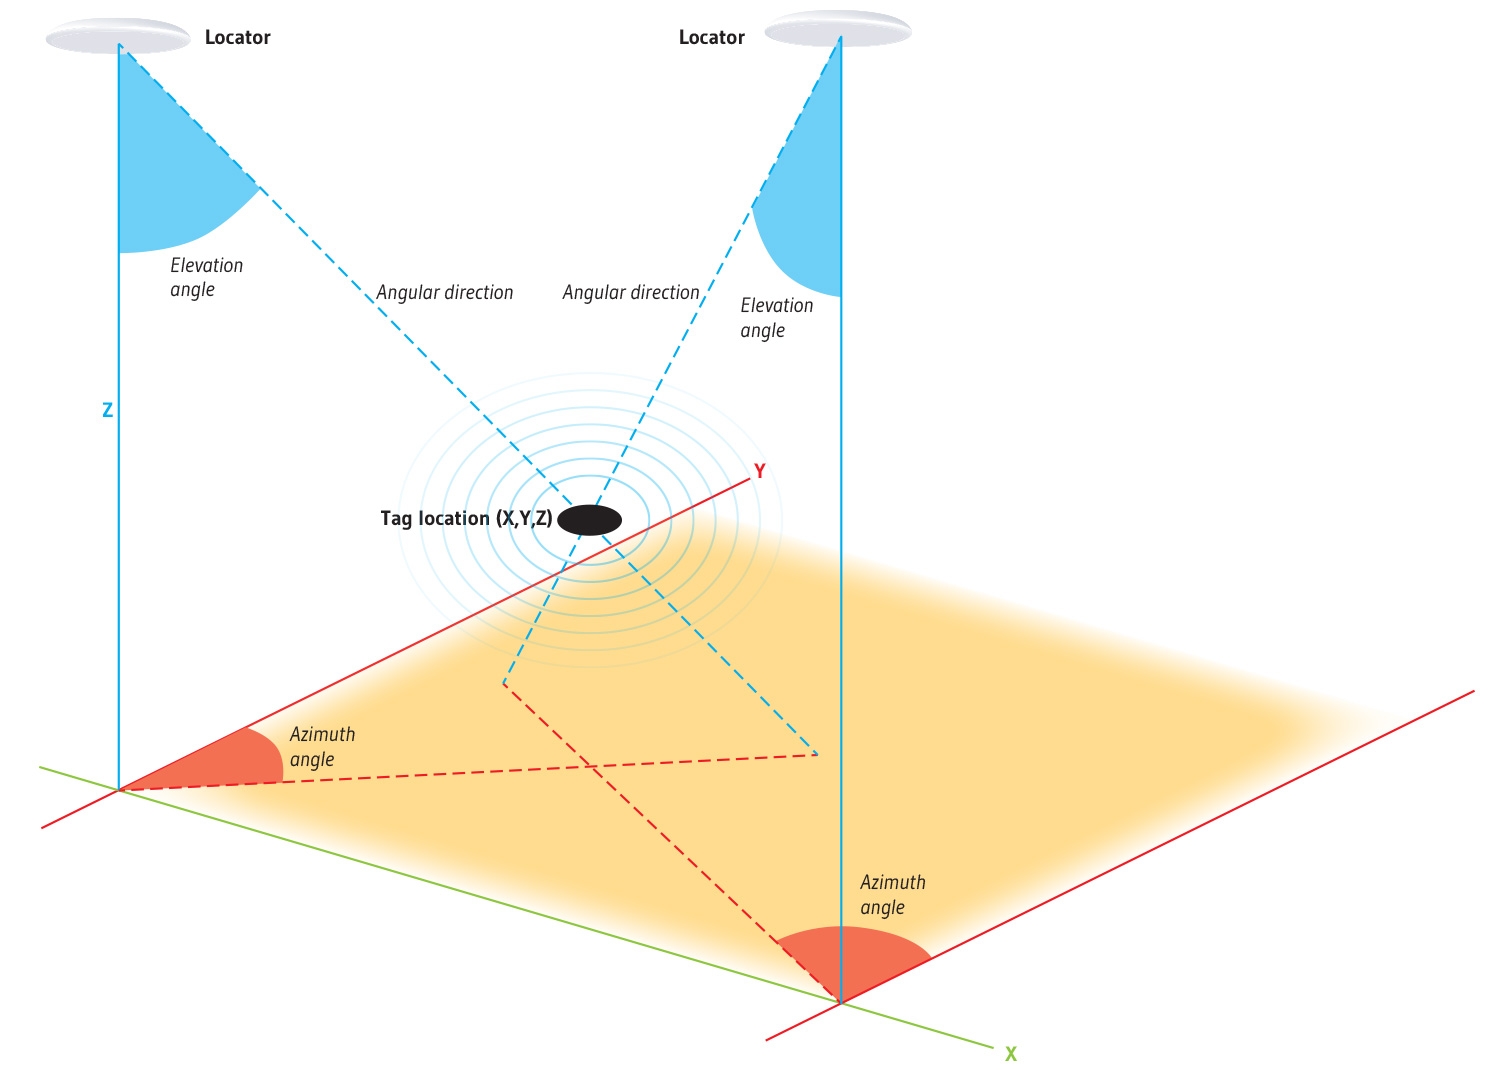
\includegraphics[width=0.6\textwidth]{img/angulation}
		\par\end{centering}
	\caption{3D location using AoA from Quuppa Intelligent Locating System (source: \cite{QAoA})\label{fig:AoAQuuppa}}
	\label{fig4}
\end{figure}

\section{Fingerprinting}\label{sec:Fingerprinting}
This method is a part of Signal Strength Fingerprint Maps (SSFM) type. Main point of this approach is using previously recorded data to figure out device location. Hence fingerprint term in the name. There is multiple kinds of radio signal sources like bluetooth, wireless or cellular devices that can be recorded.

Fingerprinting has two main phases where the first one is fingerprint maps construction also called offline phase. They are created by collecting Received Signal Strength (RSS) and optional extra features in known locations. All these values are saved in the database and it is called fingerprint map. The second phase is localization itself also known as online phase where the device measures RSS values and compares them with fingerprint maps to approximate position using suitable method \cite{LocalizationApproaches, ILWTP}. Most used algorithms or methods to approximate position are \cite{IILUBLEB}

\begin{itemize}
	\item probabilistic methods,
	\item k-Nearest Neighbors,
	\item neural networks,
	\item support vector machine,
	\item smallest M-vertex polygon.
\end{itemize}

There are multiple advantages of this approach and the most important is that it does not need any additional or specialized hardware. Next one is no need for time synchronization between the stations. Both of these advantages make it simple and cost effective method for localization. On the other hand building of the map is very time consuming and needs heavy calibration. It is also susceptible to changes in environment like people presence, object movement or relative humidity \cite{IILUBLEB, RSSFofIFD}.

\section{Proximity}\label{sec:Proximity}
Proximity detection also known as connectivity based positioning calculates only approximate location. Position is determined by cell of origin (CoO) method with known position and limited range \cite{RAinWILTaS}. Specific device location is based on cell of the connected device ("associated access point" in Wi-Fi 802.11 systems) as shown in \fref{fig5} \cite{WiFiLBS}.

\begin{figure}[h!]
	\begin{centering}
		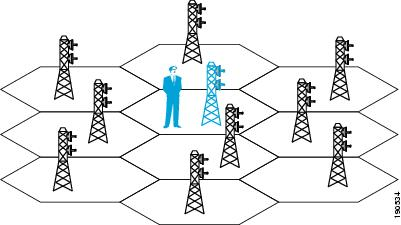
\includegraphics[width=0.6\textwidth]{img/cell_of_origin}
		\par\end{centering}
	\caption{Cell of Origin (source: \cite{WiFiLBS})\label{fig:CellOfOrigin}}
	\label{fig5}
\end{figure}

Primary advantage of this approach is very easy implementation and no need for complicated algorithms and thus making calculations fast. However, for various reasons devices can be associated to cells that are not in close physical proximity. Such errors can happen for example in multi-floor buildings where floor cells overlap. There are additional methods that can be used to improve localization such as using received signal strength indication (RSSI), manual method (human search) or connecting to device with highest signal strength \cite{WiFiLBS, RAinWILTaS}.

\section{Other techniques}
\textbf{Scene analysis} is a pattern recognition method that uses features of a scene observed from a particular vantage point to draw conclusions about the location of the observer or of objects in the scene also \cite{LSfUC}. This approach has been used in many applications, such as image and speech recognition, as well as location \cite{LSAWIFI}. The advantage is that the location of objects can be inferred using passive observation and features. The disadvantage is that the observer needs to have access to the features of environment against which it will compare its observed scenes \cite{LSfUC}.

\medskip

\textbf{Dead Reckoning} refers to a position solution that is obtained by measuring or deducing displacements from a known starting point in accordance with motion of the user \cite{DRNS}. Basically calculate new position based on starting point, travel distance and angle of movement. Because new position calculations are dependent on previous ones there is the need for high accuracy of data since it makes errors cumulative \cite{IDRAIP}.